\section{Estrazione dei Documenti}\label{sec:estrazione_documenti}
La fase iniziale della pipeline prevede l'estrazione del testo dai documenti normativi in formato PDF. 

Nelle prime fasi di sviluppo del progetto, l'intero documento PDF veniva passato direttamente al Large Language Model, demandando a quest'ultimo sia il compito di estrazione del testo grezzo sia quello di strutturazione sintattica. Questo approccio presentava forti criticità, esponeva il sistema al rischio di allucinazioni ed era inefficiente nel parsing di strutture complesse. Per superare tali limitazioni, la pipeline è stata modificata separando nettamente l'estrazione del testo dalla sua successiva strutturazione.

\subsection{Open Data Loader e la Gestione dei Tagged PDF}

Per l'estrazione del testo da documenti digitali nativi è stata adottata la libreria open-source \textit{Open Data Loader}. Questo strumento converte localmente i file PDF in formati ottimizzati per i LLM, specificamente Markdown. Il vantaggio di questa soluzione risiede nella sua natura deterministica: a parità di input viene garantito il medesimo output, azzerando le variabilità tipiche dei modelli generativi.

Durante l'analisi dei documenti legali, una delle criticità maggiori riguarda i ritorni a capo spuri, generati per ragioni puramente stilistiche (ad esempio, il raggiungimento del margine della pagina). Se non gestiti correttamente, questi si traducono in doppi ritorni a capo nel testo Markdown finale, frammentando artificialmente i periodi e compromettendo la qualità della successiva fase di chunking. Per risolvere questa criticità alla radice, l'estrazione è stata configurata abilitando il parametro specifico \texttt{use\_struct\_tree=True}.

Quando questo parametro è attivo, la libreria modifica il suo approccio di lettura, verificando innanzitutto se il file analizzato appartiene alla categoria dei \textit{Tagged PDF}. A differenza dei PDF standard, che definiscono esclusivamente il layout bidimensionale e visivo, i Tagged PDF incorporano un livello gerarchico logico e invisibile: il \textit{Logical Structure Tree}. Questo albero organizza il contenuto tramite elementi strutturali del tutto simili ai tag HTML (come \texttt{<H1>}, \texttt{<P>}, \texttt{<Table>}, \texttt{<L>}). 

Di conseguenza, abilitando \texttt{use\_struct\_tree=True}, \textit{Open Data Loader} è in grado di ignorare le fallaci euristiche geometriche e navigare direttamente la struttura logica del documento. Questo meccanismo permette all'estrattore di mappare ogni porzione di testo discriminando con precisione assoluta i semplici a capo visivi dalle reali interruzioni di paragrafo, restituendo un flusso di testo continuo e fedele all'originale.

Nel contesto della pubblica amministrazione, la formazione di documenti digitali adeguatamente strutturati non costituisce soltanto un'esigenza tecnica. L’articolo 40, comma 1, del Codice dell’Amministrazione Digitale (Decreto Legislativo 7 marzo 2005, n. 82), stabilisce infatti che \textquote{le pubbliche amministrazioni formano gli originali dei propri documenti [...] con mezzi informatici} \cite{cad_art40}.

Le modalità di formazione e gestione di tali documenti sono ulteriormente disciplinate dalle \textit{Linee guida sulla formazione, gestione e conservazione dei documenti informatici}, emanate dall'Agenzia per l'Italia Digitale ai sensi dell'articolo 71 del CAD \cite{agid_documenti_informatici}. In particolare, l'Allegato 2, dedicato ai formati di file, raccomanda di privilegiare formati \textquote{aperti, non proprietari, standard de iure, estendibili, parlanti, completamente robusti, indipendenti dal dispositivo} \cite{agid_formati_file}. Tali caratteristiche favoriscono l'interoperabilità, la conservazione nel tempo e il trattamento automatico dei documenti.

Nel caso dei file PDF, una struttura logica correttamente definita consente di rappresentare l'ordine di lettura e il ruolo semantico di elementi quali titoli, paragrafi, elenchi e tabelle. Quando presente, il \textit{Logical Structure Tree} costituisce inoltre per la pipeline sviluppata una fonte di informazioni pre-strutturate, utilizzabile per ricostruire con maggiore precisione la gerarchia e la sequenza logica del contenuto.


\subsection{Docling e l'Integrazione dei Motori OCR}

L'approccio standard basato su Open Data Loader mostra evidenti limiti in presenza di documenti non strutturati, con layout complessi o derivanti da scansioni visive, in quanto tale libreria non integra nativamente alcun modulo OCR. Per sopperire a questa mancanza è stata introdotta nel sistema la libreria \textit{Docling}. 

A differenza di Open Data Loader, Docling supporta l'integrazione diretta di motori OCR, configurandosi come un sistema avanzato di parsing e analisi del layout. Questo strumento, specializzato nell'estrazione di metadati, tabelle e testo da formati eterogenei, è stato quindi affiancato a Open Data Loader all'interno della pipeline, intervenendo come supporto specifico per processare tutti quei documenti in cui la sola estrazione con Open Data Loader risulta impossibile o inefficace.

L'introduzione dell'OCR ha sollevato complessità non trascurabili relative alla gestione delle risorse hardware all'interno dell'architettura a container. Il container Docker deputato all'estrazione operava infatti in condizioni in cui non poteva sprecare troppa RAM, date le risorse hardware limitate. Durante i primi test, l'invio massivo di interi documenti scansionati causava la saturazione istantanea della memoria, provocando l'intervento del modulo del kernel Linux (\textit{Out-Of-Memory Killer}) che terminava forzatamente il container.

Per superare il problema del consumo di RAM e prevenire i crash di sistema, è stata implementata una strategia basata sull'elaborazione pagina-per-pagina. Come discusso nel Capitolo \ref{chap:second} relativo alle scelte tecnologiche, a seguito di un'analisi comparativa dei motori supportati da Docling, la scelta è ricaduta su \textbf{RapidOCR}. Questo motore ha permesso di mantenere il consumo di memoria adeguato per il funzionamento del container, garantendo l'accuratezza del riconoscimento sul testo legale italiano.

\subsection{Progettazione del Custom Triage Processor}
Il processore di triage nativo di Open Data Loader prevede un flusso standard in cui ogni pagina viene analizzata e smistata: le pagine semplici vengono processate tramite il processo di Open Data Loader (una JVM), mentre le pagine complesse vengono delegate al backend basato su Docling. 

Tuttavia, l'applicazione con l'uso del parametro \texttt{use\_struct\_tree=True} introduce un bug logico nel triage di default: i documenti non espressamente \textit{tagged} vengono forzati all'interno del processo standard di Open Data Loader, non venendo mai instradati verso il backend di Docling, escludendo così l'analisi per pagine troppo complesse oppure l'attivazione dell'OCR dove necessario.

Per risolvere questa problematica è stato progettato e implementato un \textbf{Custom Triage Processor}. Come illustrato nel diagramma di flusso in \textbf{Figura \ref{fig:triage-processor}}, il componente corregge le anomalie di instradamento agendo secondo una logica a tre fasi:

\begin{itemize}
    \item \textbf{Fase 1: Verifica preliminare della struttura.} 
    Il file PDF viene acquisito e il sistema ne analizza i metadati per verificare se è codificato come \textit{Tagged PDF}. In caso affermativo, l'intero documento viene elaborato direttamente da Open Data Loader sfruttando l'albero strutturale nativo. Questo approccio garantisce la massima velocità di esecuzione e una pulizia ottimale del testo estratto.
    
    \item \textbf{Fase 2: Frazionamento del documento e stima della complessità.} 
    Se il documento risulta privo di struttura (\textit{Non-Tagged}), il flusso prevede la divisione in singole pagine indipendenti. Questa separazione è fondamentale per prevenire sovraccarichi di memoria RAM durante le elaborazioni successive. Per ciascuna pagina, il sistema calcola poi la densità dei caratteri testuali per valutarne il grado di complessità.
    
    \item \textbf{Fase 3: Triage ed elaborazione mirata della pagina.} 
    Sulla base dell'analisi precedente, ogni singola pagina subisce il processo di smistamento intelligente mostrato nella parte inferiore della Figura \ref{fig:triage-processor}, venendo indirizzata allo strumento di estrazione più adeguato:
    \begin{itemize}
        \item Se la pagina presenta un layout lineare e un'elevata densità di testo nativo, viene classificata come \textit{Semplice} e affidata al processo di Open Data Loader.
        \item Se la pagina contiene elementi geometrici articolati o tabelle annidate, ma il testo rimane comunque selezionabile, viene classificata come \textit{Complessa} e processata tramite Docling Standard (senza abilitare l'OCR).
        \item Se la pagina è priva di testo nativo (es. una fotocopia), viene classificata come \textit{Scansione} e inviata al container specializzato di Docling, dove interviene il motore RapidOCR per il riconoscimento ottico dei caratteri.
    \end{itemize}
\end{itemize}

\begin{figure}[H]
    \centering
    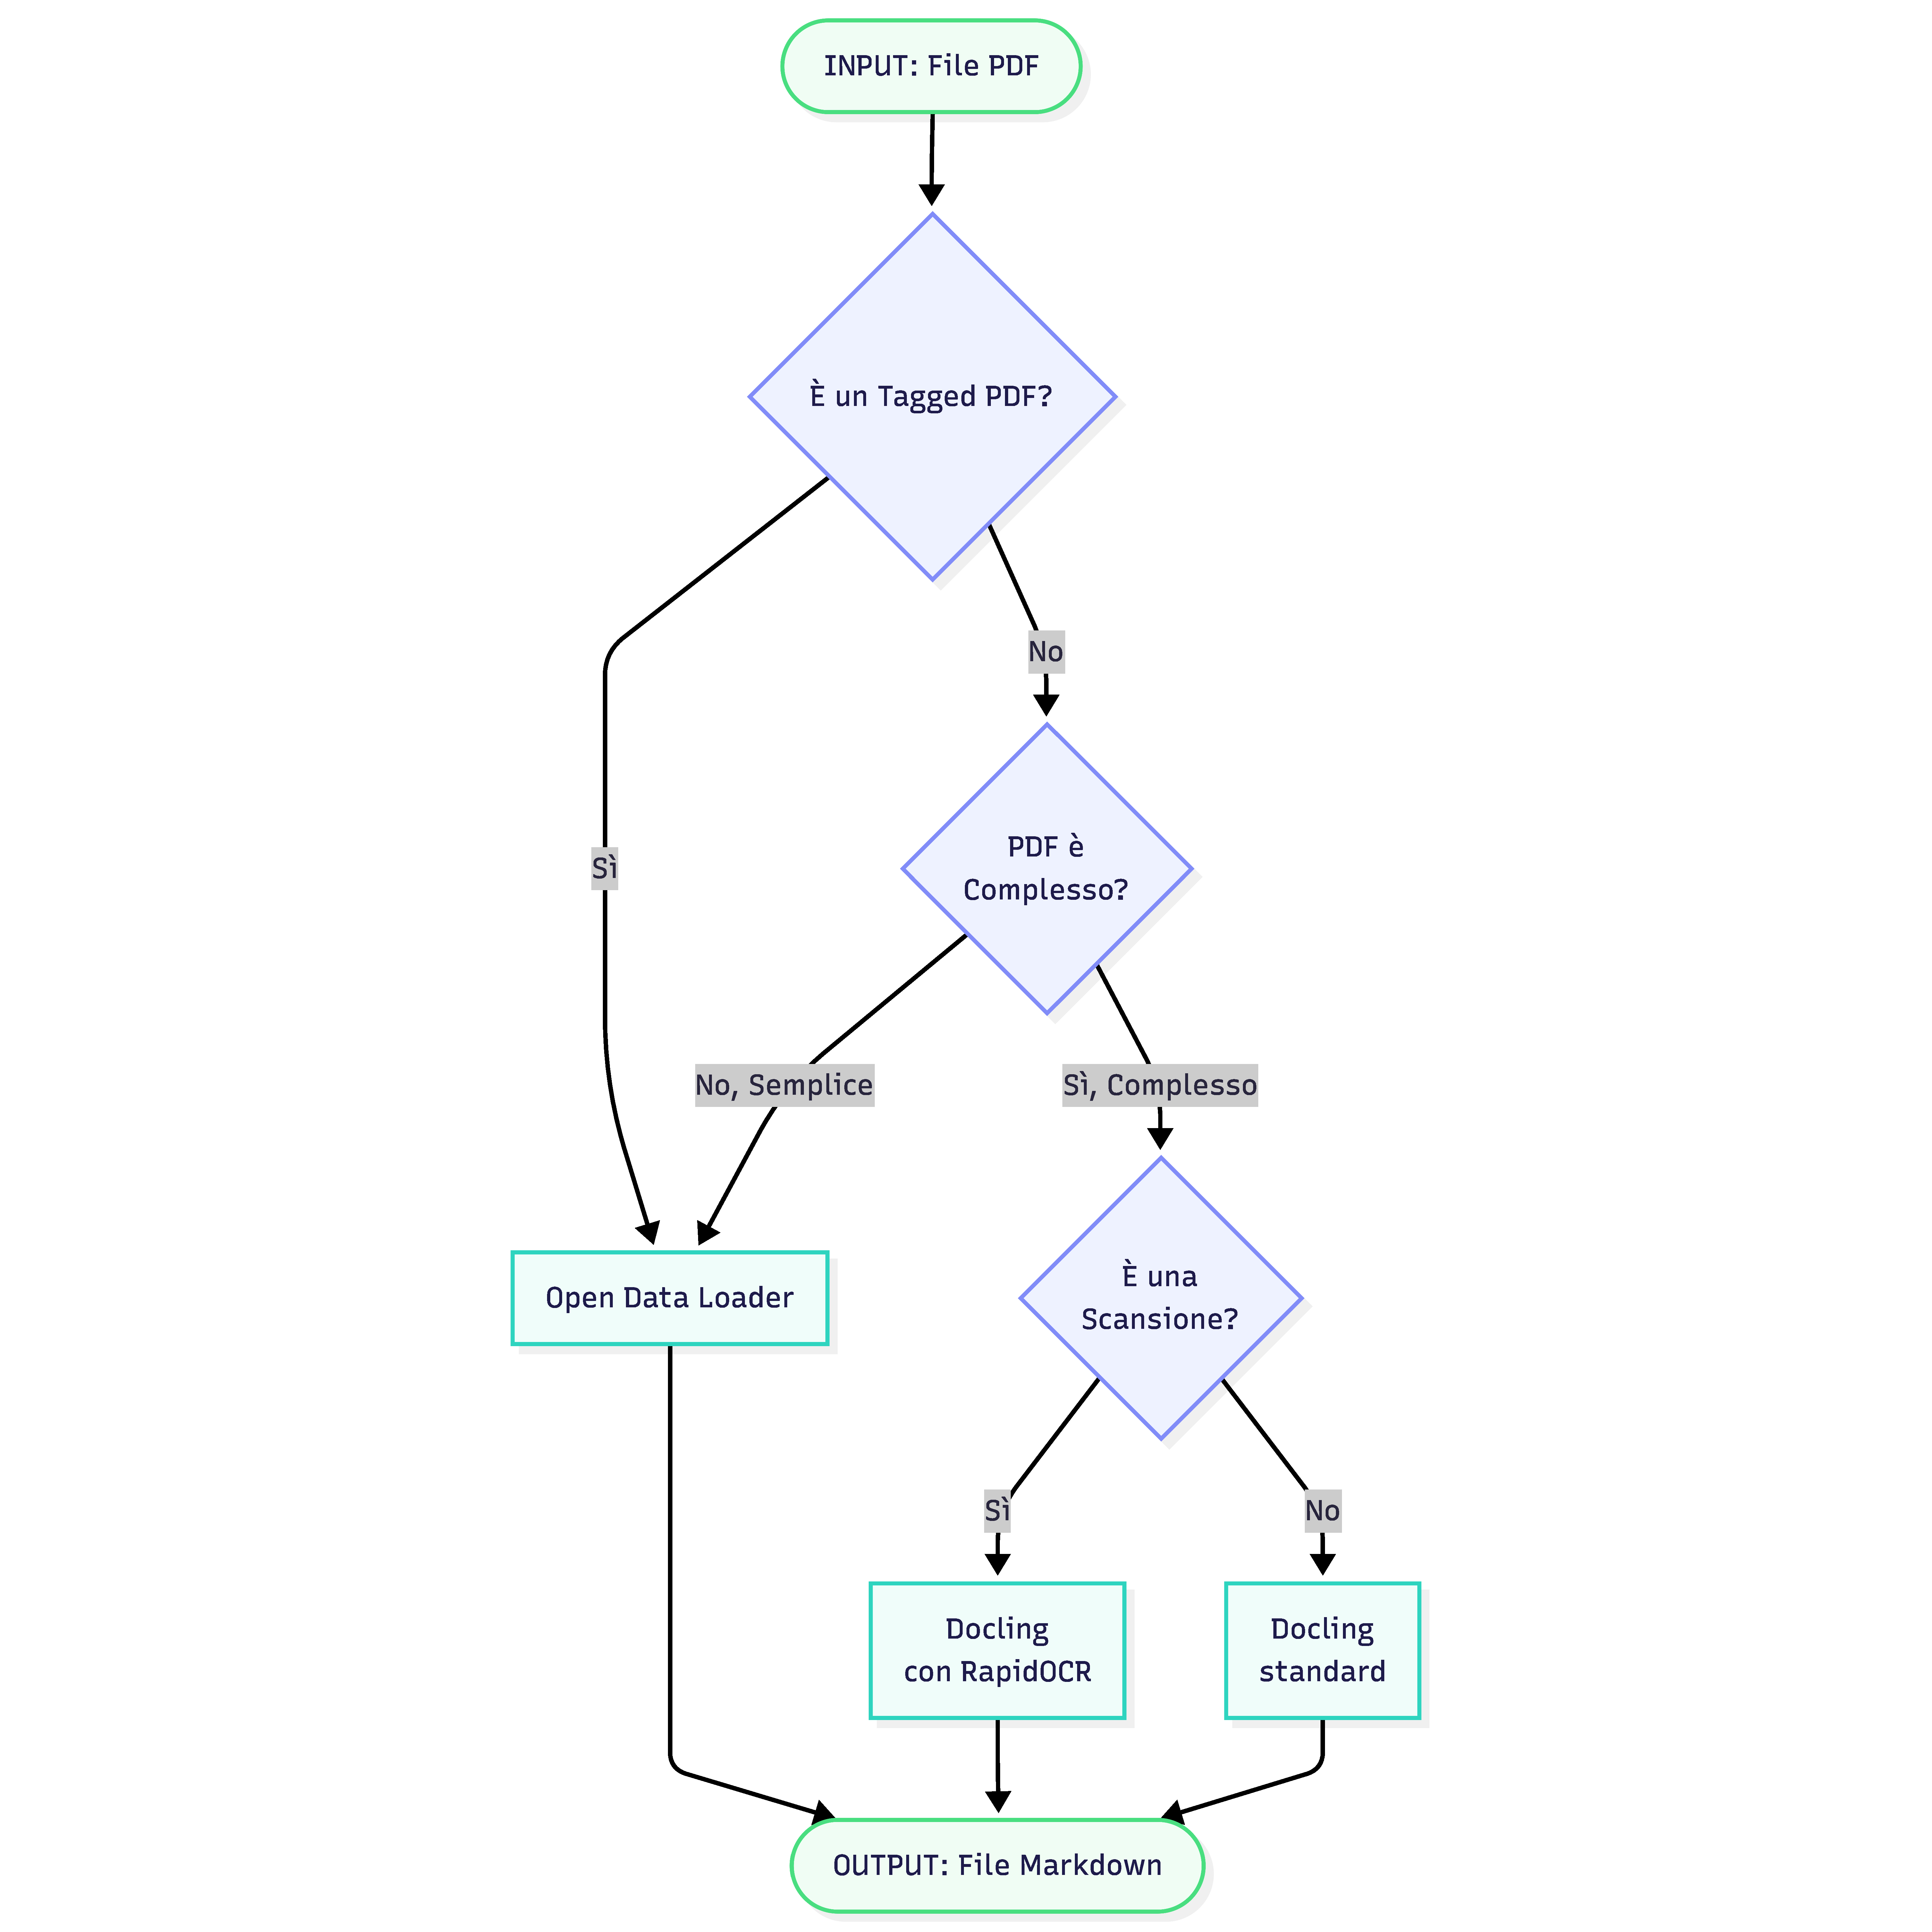
\includegraphics[width=1\textwidth]{_images/triage-processor.pdf}
    \caption{Flowchart del Custom Triage Processor}
    \label{fig:triage-processor}
\end{figure}
\newpage
